\chapter{Implementation and Experiment}
\label{chp:implexperiment}
In the previous chapter, we discussed the credit mining system design. The system can be implemented in any language with any interpretation of implementation. In this work, credit mining system implemented in Tribler, a python torrent client that was built in Delft University of Technology. Based on this implementation, we come up with the suitable experiment design to answer our research question in previous chapter. 

This chapter consists of the elaboration of both implementation and its experiment execution plan. First, in section \ref{section:triblerintregration}, we will describe how the credit mining system is implemented within Tribler. As Tribler already had a rule for new system that will be integrated, we addressed those rules. We will also look into the challenges that might be faced if Tribler deploy with credit mining system implemented and discuss the possible solution afterwards. After that, we introduce \textit{gumby} on section \ref{section:gumby}, the experiment runner developed by Tribler team in-house. The section \ref{section:cmexp} will follow to explain the actual experiment execution plan. Section \ref{section:cmparamexp} extend those experiments to an extend which it can be configurable in several points.

\section{Tribler integration}
\label{section:triblerintregration}
As a proof of concept, credit mining system was implemented as a module in Tribler. Tribler was built using python, compatible with version 2.x and 3.x. At the time credit mining system implemented in Tribler, Tribler stil use WX as GUI (Graphical User Interface) framework. As for the future, Tribler will move its GUI to use Qt, starting version 7.0 onwards. All of those components made Tribler work cross platform (Linux, MacOS, and Windows).

In the prior work, some of the credit mining system code were implemented by \citeauthor{2015:creditmining:capota} and Egbert Bouman in his Tribler fork\footnote{\url{https://github.com/mihaic/tribler/tree/channel_boosting_new_exp}} instead of the main repository. This made the compatibility and stability between Tribler and credit mining system broke, thus make the system unusable. At this stage, the credit mining code was 1528 line long with 51 deletions.

% implemented in wx for GUI
\subsection{Contribution on software engineering}
As part of the software engineering process, the credit mining code need to be pass several steps before merged into main repository. First and foremost, is to open a Pull Request from forked repository to main. In Tribler, there are two main branch : \texttt{devel} for all new features and fixes, and \texttt{next} which contains bug fixes for the stable release. The pull request of first credit mining prototype was directed to \texttt{devel} branch as it is new feature at that point. Next phase is to work on the code itself by committing the work to the pull request. After that, other member of Tribler will review the implementation. One of the review material is the auto test report that executed by Jenkins\footnote{\url{http://jenkins.tribler.org/}}. The peer review process repeated until no other feedbacks. The lead developer will do a final review afterwards. After they gave OK sign, the commits need to be squashed and finally the pull request can be merged. Figure \ref{fig:cmpullrequest} shows the pull request that has been merged into Tribler main repository on \texttt{devel}.

\begin{figure}[h]
	\centering
	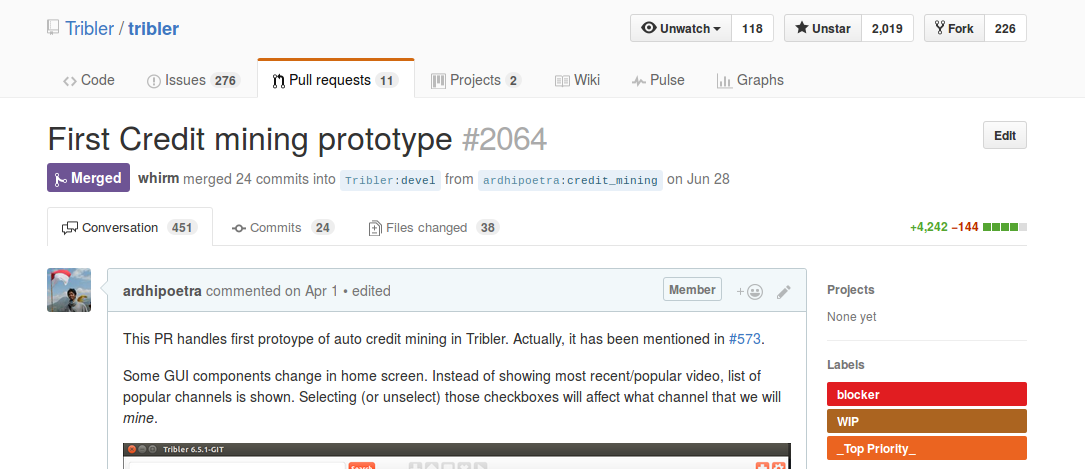
\includegraphics[width=\textwidth]{pics/cm_pr_crop.png}
	\caption[Merged pull request on credit mining prototype]{Merged pull request on credit mining prototype\footnotemark.}
	\label{fig:cmpullrequest}
\end{figure}

As shown in Figure \ref{fig:cmpullrequest}, the first credit mining prototype was heavily discussed by 6 other participants and more than 450 comments. It also takes almost 3 months to accommodate all the feedbacks and reviews. The coverage of this integration worth more than 4200 added lines and 140 deletions. The code portion is quite balanced with 1425 lines goes to GUI part of the code, 1290 lines to the credit mining system itself, 1160 lines to the tests, while the rest to other Tribler components to accommodate credit mining system. At the time of merging, credit mining system passed all the necessary test such and able to run in Linux, MacOS, and Windows (both 32 and 64 bit).

\footnotetext{Available in : \url{https://github.com/Tribler/tribler/pull/2064/}}
\subsection{Experience enhancement}
Credit mining system implementation is made publicly available for end user. It is important to encourage user to be as altruistic as possible. Therefore, in this system, we provide minimal interaction so non-altruistic user can be shown the effect of altruism and be convinced that this behavior is beneficial for both parties. In this part, we will elaborate the effort we have done on enhancing user experience of credit mining system on Tribler. As for comparison, Figure \ref{fig:oldcm} shows the only interface available from the previous work. In this version, it was not possible to add the mining sources except from the Tribler configuration file. 

\begin{figure}[h]
	\centering
	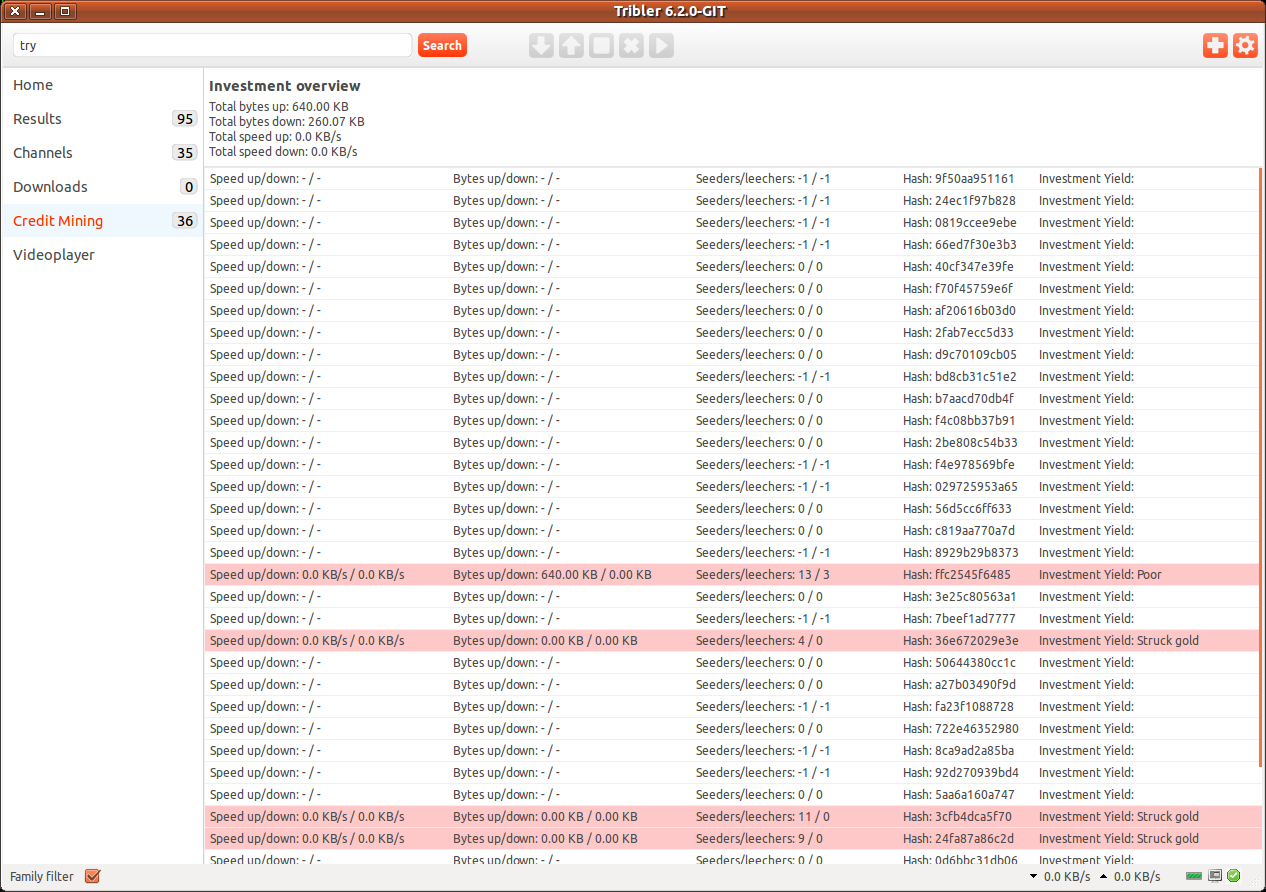
\includegraphics[width=0.8\textwidth]{pics/old_cm.png}
	\caption{The GUI for showing information from prior work \cite{2015:creditmining:capota}.}
	\label{fig:oldcm}
\end{figure}

\subsubsection{Graphical user interface revampment}

Start with the screen we called credit mining main window, it has similar interface compared with previous version. We improved the investment summary by adding more information of the mining source. The investment summary screen contains the swarms download/upload speed, amount of downloaded/uploaded, amount of seeder/leecher, and its identification. Figure \ref{fig:overview} shows this screen. In the same window, we also integrate an interface to easily add or remove mining sources. As mentioned in Section \ref{section:msource}, currently there are only 3 types of sources. Adding RSS and directory source can be done by clicking the upper left option. In the other hand, adding channel source can be done by put the mark in the check boxes in the source list. Figure \ref{fig:addsource} shows the example of adding directory source.

\begin{figure}[t!]
	\begin{adjustwidth}{-2.5cm}{}
		\begin{subfigure}[t]{0.6\textwidth}
			\centering
			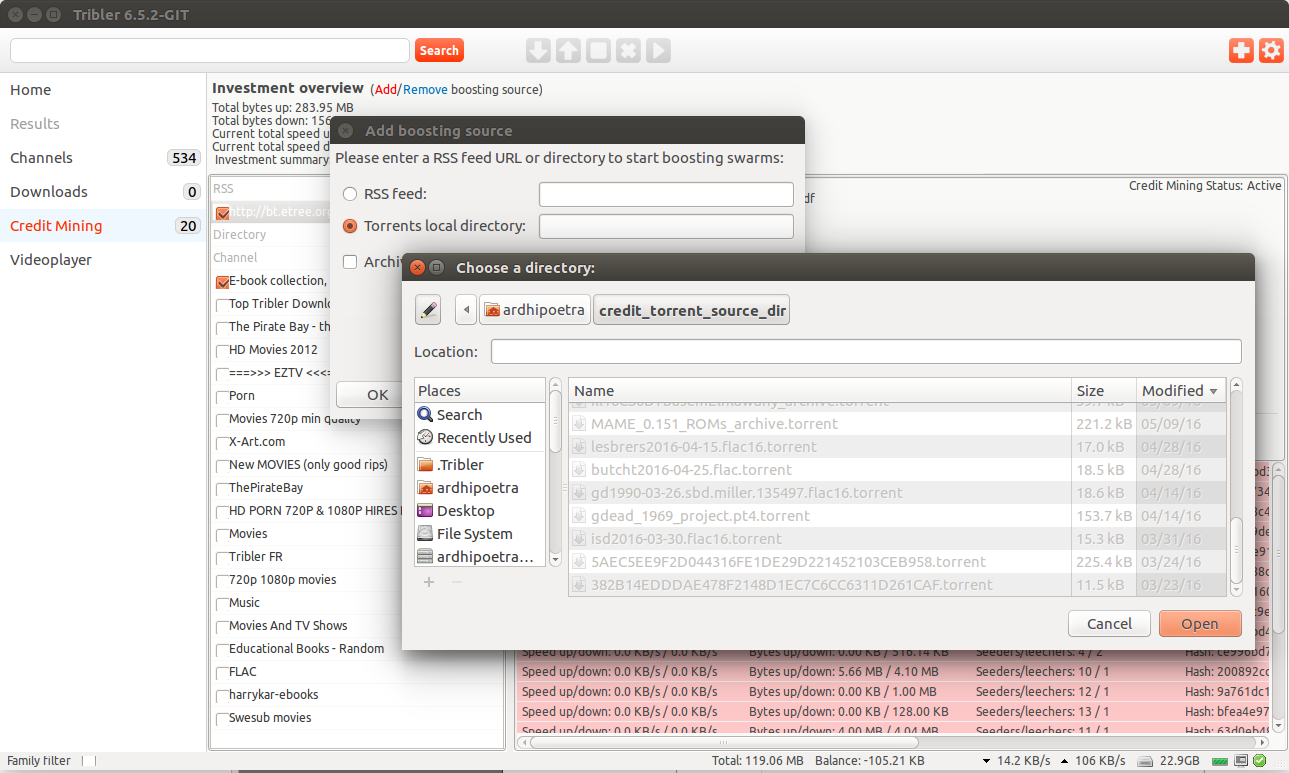
\includegraphics[width=\textwidth, height=6cm]{pics/add_source.png}
			\caption{The interface of adding mining source.}
			\label{fig:addsource}
		\end{subfigure}
		~
		\begin{subfigure}[t]{0.8\textwidth}
			\centering
			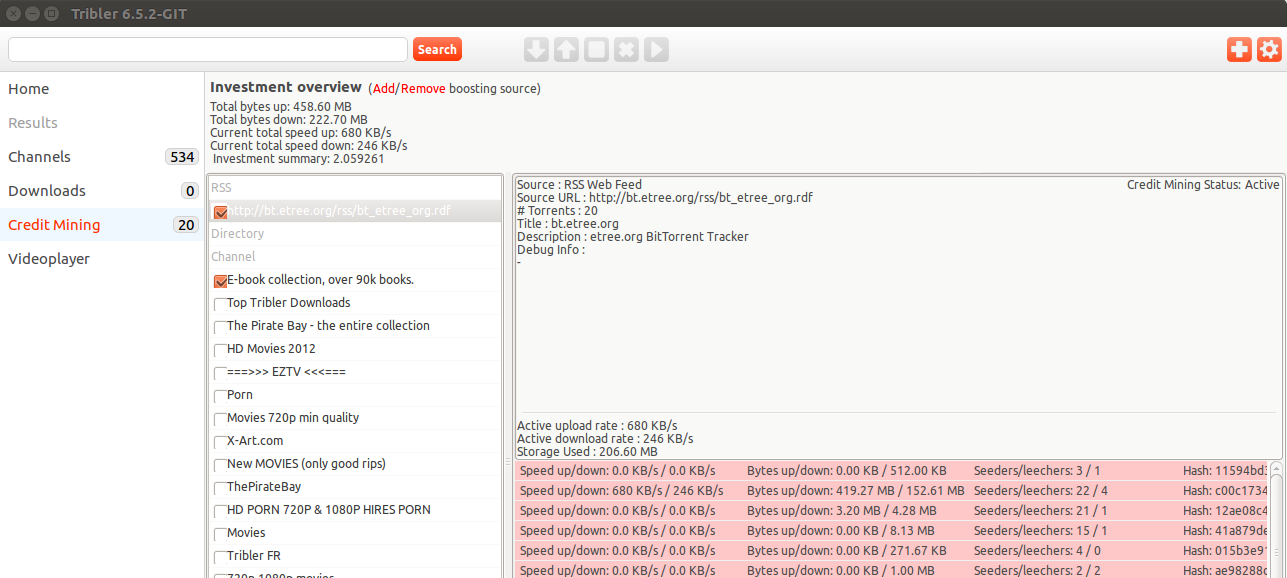
\includegraphics[width=\textwidth, height=6cm]{pics/overview_result.png}
			\caption{The investment overview.}
			\label{fig:overview}
		\end{subfigure}
		\caption{Credit mining main window.}
	\end{adjustwidth}
\end{figure}

Credit mining system is disabled by default in Tribler. Because it relates with automatically upload data, it might be concerned with privacy and security issue on end users. Therefore, a user must opt-in to enable credit mining. It can be done by flag the checkbox in Tribler settings window. After enabled, user need to restart Tribler to have the settings take effect. 

Activating credit mining module made the home screen of Tribler changed. We put several channels sorted by its popularity at the home screen as shown in Figure \ref{fig:homecm}. Channel is an integral part of Tribler which can be used to disseminate swarm information. This way, Tribler user do not need to leave the application to download new content. In home screen, user can simply click which channel he want to mine. This action will also be reflected in the credit mining main screen. To provide user with sufficient information, the popularity, shown by stars in the channel, and the random swarm that resides within that channel is showed. Moreover, user can also look for channel information if necessary. In this way, Tribler user have an easy access to mine a channel, which we strongly recommend.

\begin{figure}
	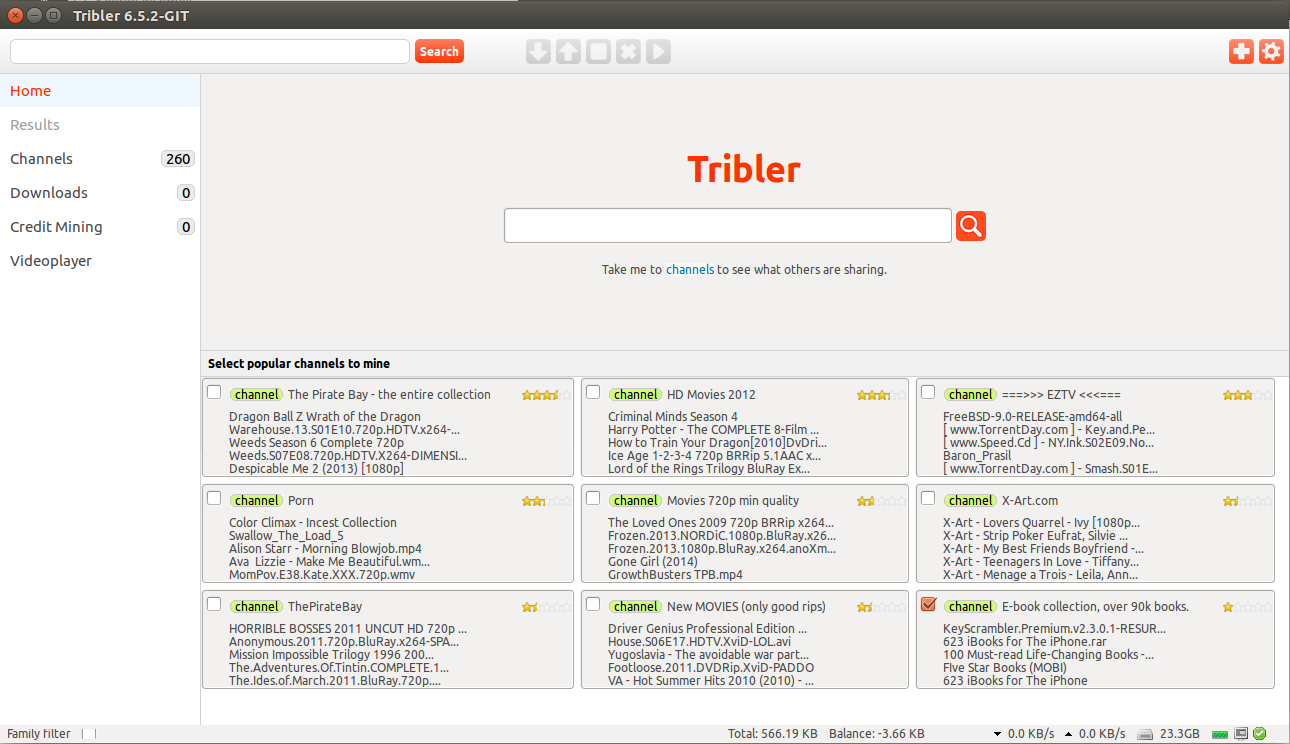
\includegraphics[width=\textwidth]{pics/home_channel.png}
	\caption{The home interface of Tribler with credit mining active.}
	\label{fig:homecm}
\end{figure}

In integrating with Tribler, we emphasize the simplicity to both interact with credit mining system and monitor gained credit. Especially to mine channel, two methods are introduced, both are by single-clicking the checkboxes in home screen (Figure \ref{fig:homecm}) or in credit mining main page (Figure \ref{fig:overview}). Although in the home screen only limited popular channel are shown, in credit mining main page this is not the case. After scrolled some content, if Tribler find another channel that has not been shown, it will append the list with that channel. Basically, it is an infinite list of channel with the upper bound the total number of channel available in Tribler environment. After the channel has been added to credit mining system, user can enable or disable it by another single click.

\subsubsection{User activity awareness}
One important point to ensure user to keep using any system is to not disturb their activity. In a typical torrent client, non-altruistic user tend to only activate his client when downloading. Although credit mining system runs automatically, it is possible the system will find a potential swarm then actively download from it. For a user with limited bandwidth, we realize this could be a problem if this user realize his bandwidth that currently used is taken by credit mining system. In a long term, this may cause user to disable this system because of the potential intrusiveness. We define the \textit{user download activity} as the activity that intentionally initiated by user in order to participate or download content on the particular swarm. Usually, it is the true purpose of having torrent client. 

\todo{Restructure the following}In response to that issue, on the integration with Tribler, we also implemented another module in credit mining system to adjust its mining activity to user download activity. Credit mining system periodically check whether there is an user downloading activity. If there is not any, then credit mining system can notify the miners to use all the bandwidth available. If there is an activity, user need to set the priority of credit mining download activity. By default, the priority of credit mining download activity will be reduced to one-third\todo{tentative}. This means, the swarm in the user download activity will get 3 times higher probability of bandwidth allocation compared to the one in credit mining download activity. The bandwidth distribution is not strictly in order, however, the priority is used as weight for it.

%\subsubsection{Libtorrent tuning}
%settings in libtorrent to accommodate credit mining <- removed it for now.

\subsection{Anonymous and secure mining}
\todo[inline]{untested. May skip this subsection. See .tex file for draft}
%Tribler is well known for its anonymity and secure interface on top of \bt~ network. In 2014, Tribler published a specification on its anonymity feature\footnote{\url{https://github.com/Tribler/tribler/wiki/Anonymous-Downloading-and-Streaming-specifications}}. It uses Tor-like onion routing with purely distributed mechanism. A year later, \citeauthor{2015:tunnel:ruigrok} on his work completed the \textit{tunnel community} which emphasize end-to-end encryption in Tribler. This comes with several drawbacks. The most important one is performance degradation. Adding layers of privacy comes with increasing the amount of cryptography operation which slows down end-to-end downloading activity \cite{2015:tunnel:ruigrok}.

% enable safe_seeding: when finished and in 'seeding' state. hops: download/upload via libtorrent proxy.

\section{Gumby}
\label{section:gumby}
After credit mining system is integrated with Tribler, the next part is to test whether the implementation showing expected result or not. One way to conduct the experiment is by launching Tribler clients in the wild and monitor them using reporting mechanism. Another method is by create several virtual machines and launch Tribler within it. Both approaches are not scalable and very difficult to automatize. Fortunately, in Tribler, there is an experiment runner that can be used to run Tribler in both local machine or cluster to emulate the experiment.

\textit{Gumby}\footnote{\url{https://github.com/Tribler/gumby}} is an experiment runner framework for performing in both Tribler and Dispersy. Gumby can run both in local computer and cluster computer. In this case, we able to run gumby in DAS4 and DAS5 (via Jenkins) as part of our experiment. Gumby run on different scenarios that can be specified. It uses configuration file for each experiment to define all the settings needed for one run. Developer can easily specify the number of peer needed for one experiment, the post process script after running experiment, the value that needed to be distributed to all of the peers, and many others. The most important part is to code the experiment code itself written in \texttt{python}. In this file, one must define how the experiment will run and behave. How the commands interpreted also described in this file. There are some functions and classes that need to be extended to make the experiment works.

Gumby run in sequential manner with several steps. The set of steps are different depends on the flag specified in the configuration. But in general, the run is executed as follows. First, gumby read the scenario and configuration file. After deciding what type of experiment it has to run, it will clear the output directory and synchronize it on multiple nodes, in case of running it in cluster computing. Next, the setup script will be executed. It usually contains the experiment requirement that need to be built. After that, it spawns Dispersy and experiment tracker to monitor the experiment in case of error occurred. All of the experiment nodes communicate with server using specified IP and port. Server also expected to exchange messages between nodes whenever needed or specified in the scenario. Finally, both local and remote processes are started in parallel. Upon finishing experiment, server will wait all node instances to exit and disconnect. Then it will copy the data to predefined directory which can be processed using specified post-experiment script to generate items such as graphs and tables.

\subsection{Scenario and Configuration}
In gumby, it is not possible to intervene the experiment on the fly. What the developer can do is by specifying commands in scenario file. The scenario notation is quite simple. It only needs the time of an action that has to be executed and the command itself. Optionally, which node that run the command can also be specified. Figure \ref{fig:gumbyscenario} shows the example of the aforementioned scenario. For example, command \texttt{@0:36 set\_boost\_settings boosting.ini.1 \{3\}} means in seconds 36, gumby will run command \texttt{set\_boost\_settings} with \texttt{boosting.ini.1} as parameter on node number 3. 

\begin{verbbox}
@0:0 set_master_member 3081a73010...e75
@0:2 start_dispersy {1-3}
@0:10 start_session
@0:22 online
@0:23 set_speed 0 0 {3}
@0:32 create {1}
@0:35 publish file1gb_1 1524288077 {1}
@0:36 set_boost_settings boosting.ini.1 {3}
@0:37 start_boosting {3}
@0:40 add_source http://bt.etree.org/rss/bt_etree_org.rdf {3}
@1:15 start_download file1gb_1 {2}
@1:33 reset_dispersy_statistics
@0:43100 stop
\end{verbbox}

\begin{figure}[h]
	\fbox{\theverbbox}
	\caption{Scenario format example}
	\label{fig:gumbyscenario}
\end{figure}

With scenario defined as a custom format, on the other hand, gumby configuration file only contains the number of variables that need to be filled. These variables can be accessed from inside the program. Figure \ref{fig:gumbyconf} shows the example of configuration format in gumby. There are some necessary variables such as experiment name and \texttt{tracker\_cmd}. Some of the variables required by specific conditions. For example, if \texttt{local\_instance\_cmd} is \texttt{'das4\_reserve\_and\_run.sh'}, it is necessary to call the other 4 subvariables that recognized by \texttt{das4\_} precedence. Lastly, there are variables that completely optional or needed by the experiment file. In this case, specifying \texttt{scenario\_file} is optional to direct whith scenario we want to run in a single experiment.

\begin{verbbox}
experiment_name = "CreditRunner_base_DAS"
experiment_server_cmd = 'experiment_server.py'

local_setup_cmd = 'das4_setup.sh'
local_instance_cmd = 'das4_reserve_and_run.sh'

output_dir = '/var/scratch/aputra/cmining'

das4_node_amount = 2
das4_node_timeout = 3600
das4_instances_to_run = 5
das4_node_command = "creditmining.py"

tracker_cmd = 'run_tracker.sh'

use_local_venv = True

scenario_file = "creditmining_base.scenario"
post_process_cmd = "gumby/scripts/post_credit_mining.sh"
\end{verbbox}
\begin{figure}[]
%	\begin{adjustwidth}{-2cm}{}
	\fbox{\theverbbox}
	\caption{Configuration format example}
	\label{fig:gumbyconf}
%	\end{adjustwidth}
\end{figure}

\section{Credit mining experiment}
\label{section:cmexp}
The credit mining experiment covered two aspects : local and global. 

\subsection{Comparing performance with prior work}
\subsubsection{New policy}
\subsection{Predownload hit capabilities}
\subsubsection{Torrent crawler}
\subsection{Experiment on user activity}

\section{Finding best parameters}
\label{section:cmparamexp}
\subsection{Multiplier in scoring policy}
\subsection{Number of piece download}
\subsection{Peer translation accuracy}


